\section{Experimental Setup}

Bloom taxonomy evaluation compares three Qwen-related approaches against a lexical baseline on Figshare exam questions: \textbf{TF-IDF + LinearSVC}, \textbf{zero-shot Qwen2.5-1.5B GGUF} (prompt-only, no LoRA), and \textbf{fine-tuned Qwen2.5-1.5B LoRA} (\texttt{train\_qwen\_bloom.py}, \texttt{predict\_bloom.py}). Hold-out baselines use a 15\% stratified split ($n{=}379$); the deployed LoRA model is evaluated on the official audited test split ($n{=}2330$). Privacy, student QA/RAG, and multimodal OCR are evaluated separately.

Artifacts: \texttt{evaluation\_outputs/evaluation\_report.json}, \texttt{evaluation\_results/metrics.json}, \texttt{results/bloom\_baseline\_comparison.json}.

\section{Performance Metrics}

\begin{itemize}
    \item \textbf{Accuracy, macro-F1, weighted-F1} for Bloom label prediction.
    \item \textbf{Mean ordinal distance} and \textbf{within-one-level accuracy} for moderation-relevant error structure.
    \item \textbf{Severe error rate} for predictions more than one Bloom level away (baselines) or $\geq 3$ levels (LoRA script).
    \item \textbf{Cohen's $\kappa$} (hold-out baselines).
    \item Privacy, QA/RAG, and OCR metrics as in later subsections.
\end{itemize}

\section{Result Analysis}

\subsection{Bloom Taxonomy: Qwen and Baseline Comparison}

Table~\ref{tab:bloom_qwen_comparison} summarizes the current Bloom evaluation. Fine-tuned LoRA is the deployed teacher classifier; zero-shot GGUF shows that prompting alone is insufficient; TF-IDF + LinearSVC is a strong lexical baseline on the same hold-out split as zero-shot.

\begin{table}[H]
\centering
\small
\caption{Bloom classification results (current evaluation artifacts)}
\label{tab:bloom_qwen_comparison}
\setlength{\tabcolsep}{4pt}
\begin{tabular}{@{}p{2.35cm}p{1.55cm}rrrrr@{}}
\toprule
\textbf{Model} & \textbf{Split} & \textbf{Acc.} & \textbf{Macro-F1} & \textbf{Wtd-F1} & \textbf{Within-1} & \textbf{Sev.} \\
\midrule
TF-IDF + LinearSVC & 15\% hold-out & 0.839 & 0.826 & 0.838 & 0.916 & 0.084 \\
Qwen zero-shot (GGUF) & 15\% hold-out & 0.441 & 0.369 & 0.424 & 0.686 & 0.314 \\
Qwen LoRA (fine-tuned) & Official test & 0.748 & 0.721 & 0.741 & 0.880 & 0.064 \\
\bottomrule
\end{tabular}

\vspace{0.4em}
\footnotesize
\textit{Note:} Hold-out rows from \texttt{evaluation\_outputs/} ($n{=}379$); LoRA row from \texttt{evaluation\_results/metrics.json} ($n{=}2330$). Mean ordinal distance: SVM 0.322, zero-shot 1.074, LoRA 0.452. SVM vs.\ zero-shot agreement 47.5\%.
\end{table}

\begin{table}[H]
\centering
\small
\caption{Extended Bloom metrics (ordinal distance and $\kappa$)}
\label{tab:bloom_qwen_extended}
\begin{tabular}{@{}p{2.5cm}p{1.6cm}rrr@{}}
\toprule
\textbf{Model} & \textbf{Split} & \textbf{Ord.\ dist.} & \textbf{$\kappa$} & \textbf{Macro-F1} \\
\midrule
TF-IDF + LinearSVC & 15\% hold-out & 0.322 & 0.790 & 0.826 \\
Qwen zero-shot (GGUF) & 15\% hold-out & 1.074 & 0.244 & 0.369 \\
Qwen LoRA (fine-tuned) & Official test & 0.452 & --- & 0.721 \\
\bottomrule
\end{tabular}
\end{table}

Figure~\ref{fig:bloom_lora_cm} shows the LoRA confusion matrix on the official test split. Figures~\ref{fig:bloom_baselines_cm}--\ref{fig:bloom_agreement} show hold-out baseline confusion matrices and SVM vs.\ zero-shot agreement.

\begin{figure}[H]
    \centering
    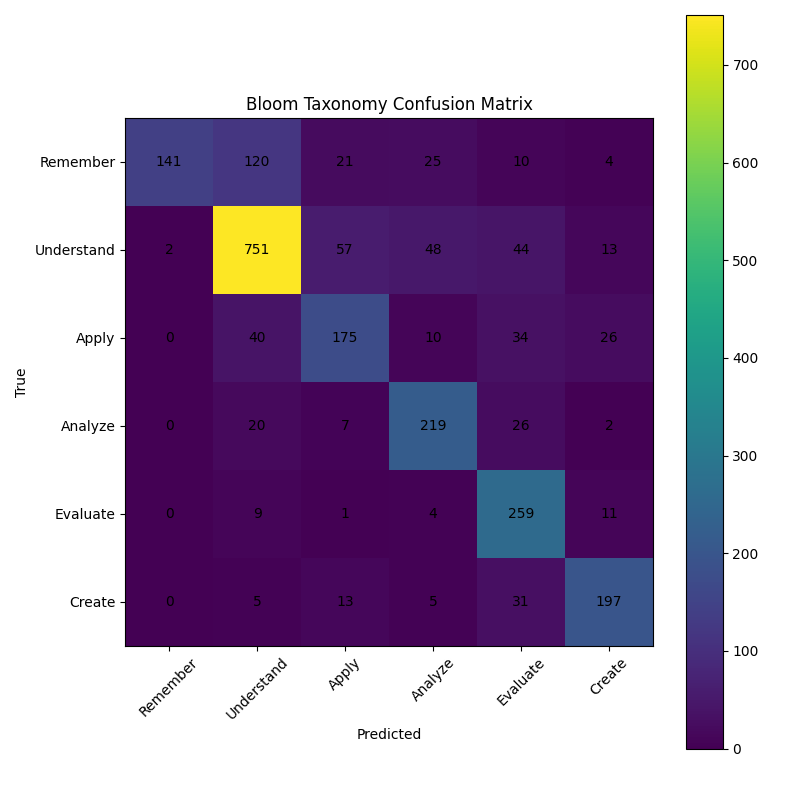
\includegraphics[width=0.75\textwidth]{images/bloom_lora_cm.png}
    \caption{Qwen2.5-1.5B LoRA confusion matrix (official test split, $n{=}2330$).}
    \label{fig:bloom_lora_cm}
\end{figure}

\begin{figure}[H]
\centering
\begin{subfigure}{0.48\textwidth}
    \centering
    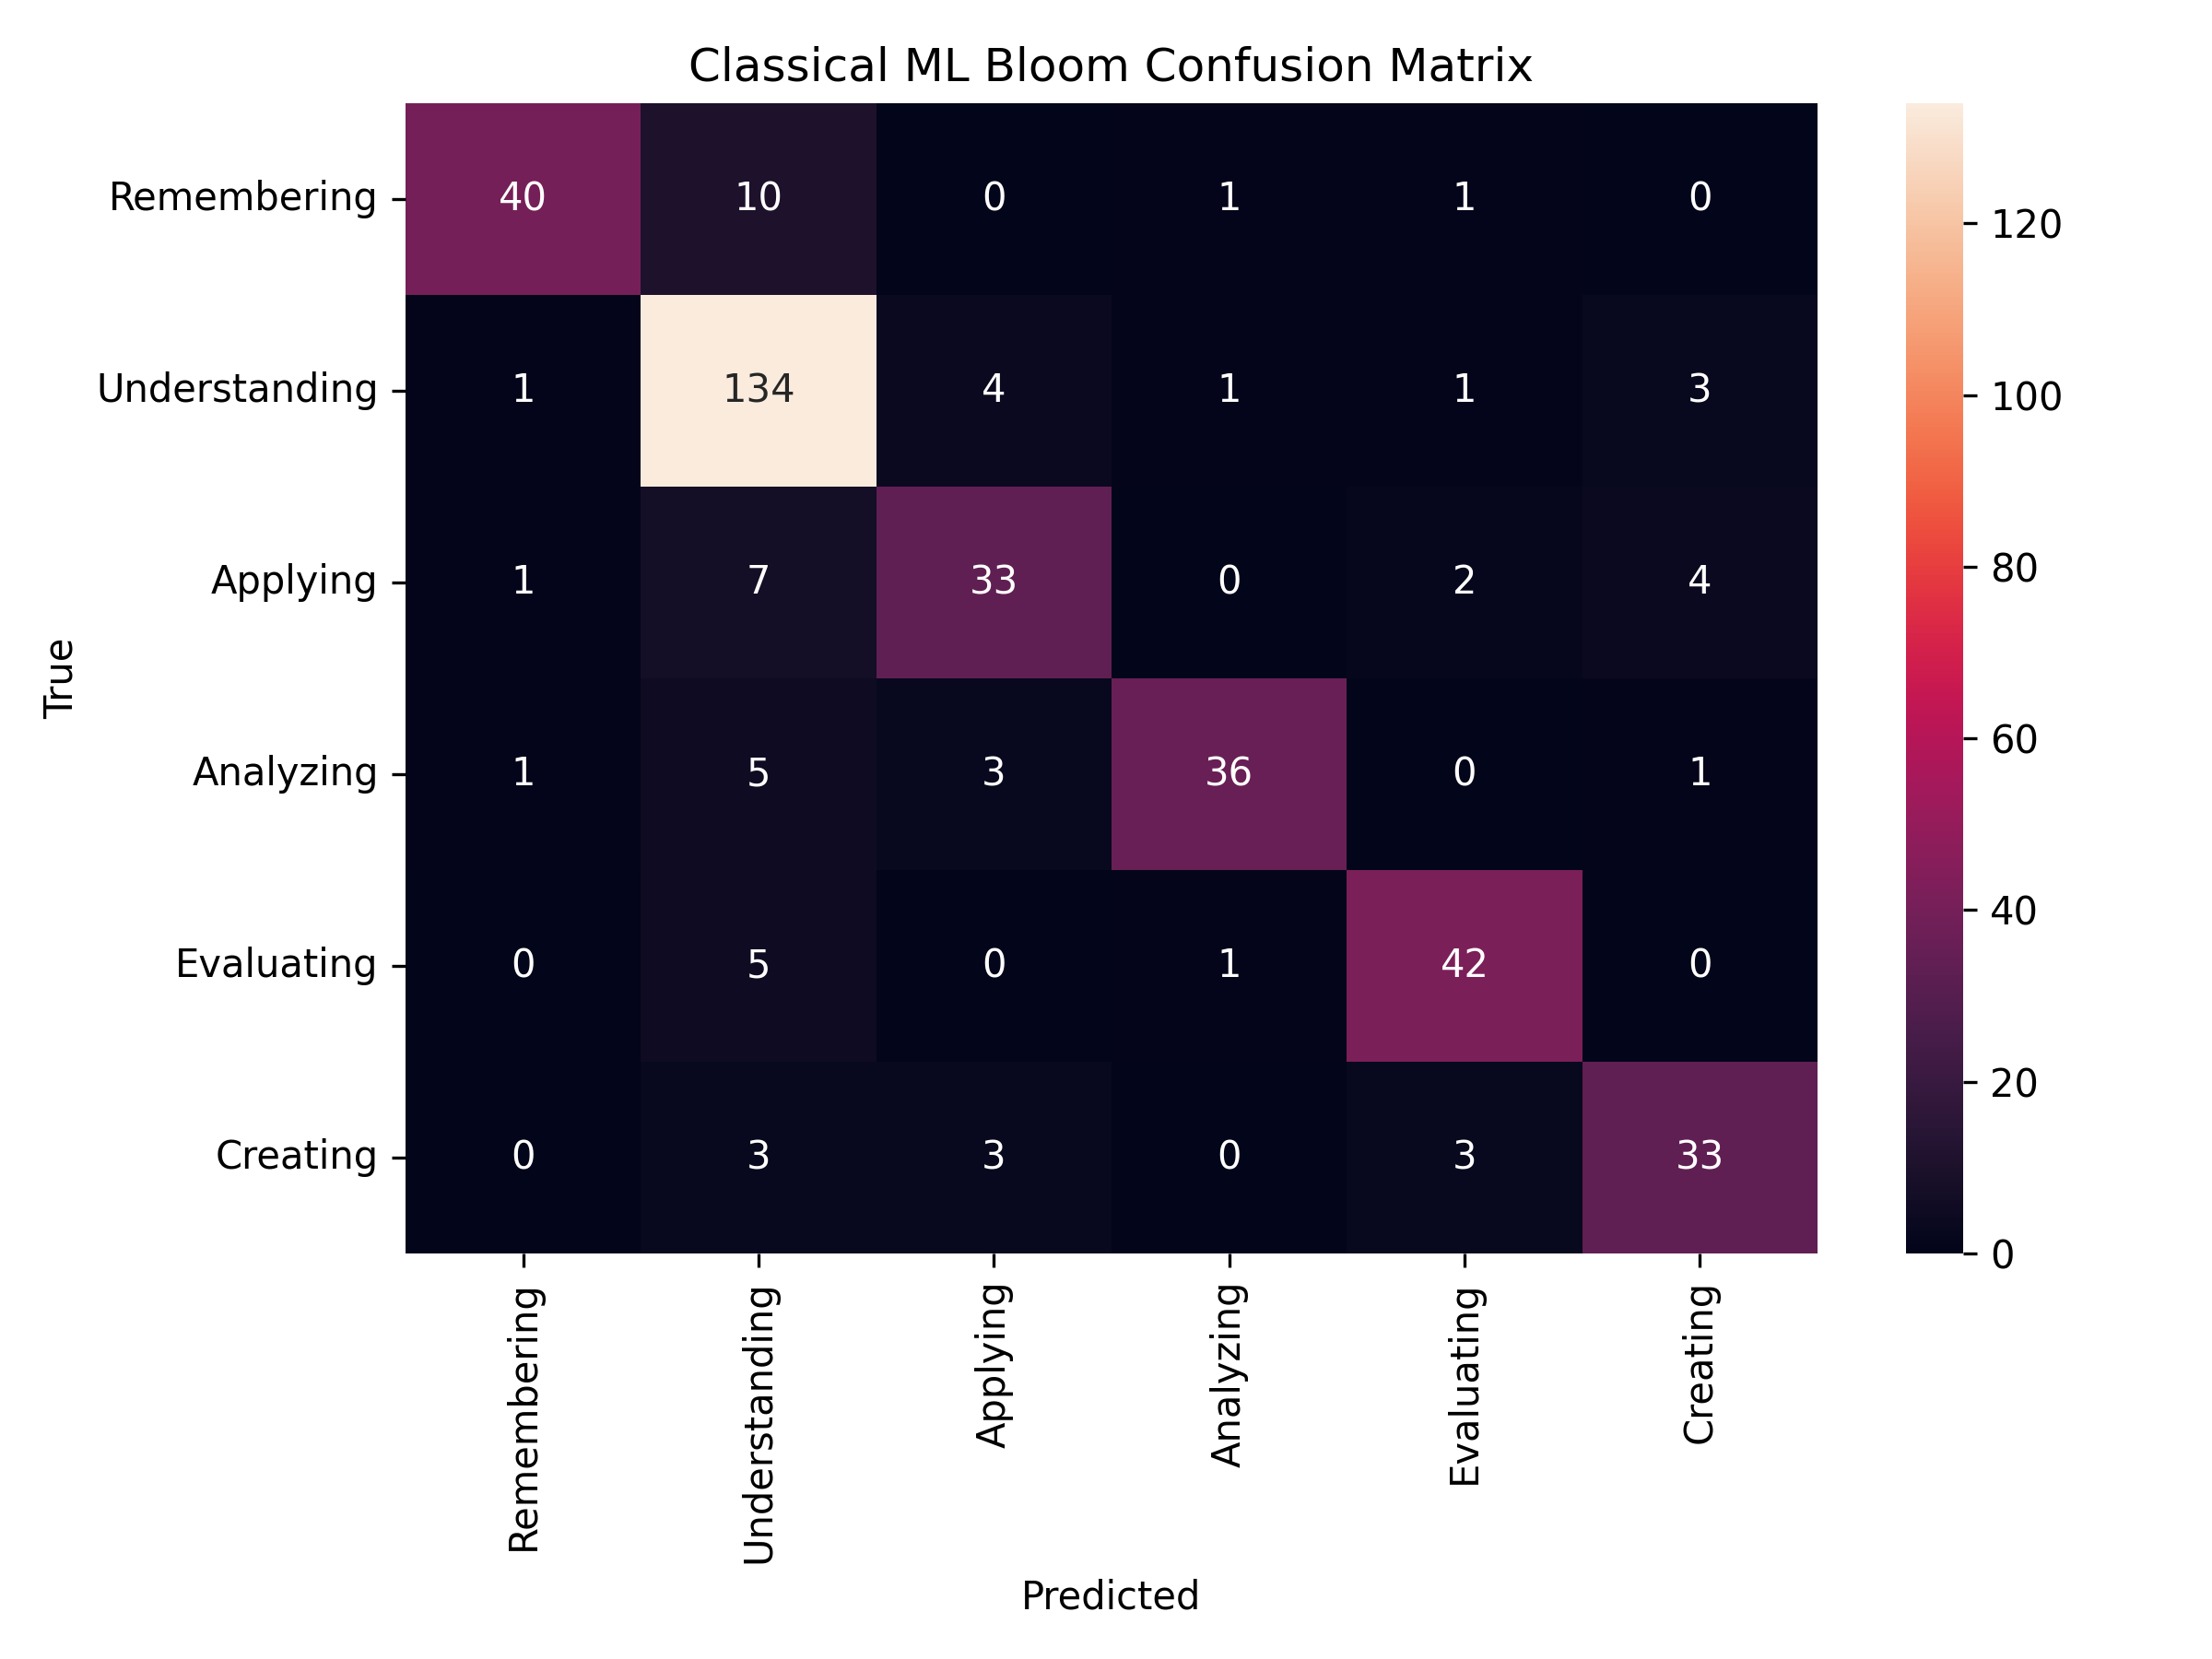
\includegraphics[width=\linewidth]{images/bloom_svm_cm.png}
    \caption{SVM (hold-out)}
\end{subfigure}
\hfill
\begin{subfigure}{0.48\textwidth}
    \centering
    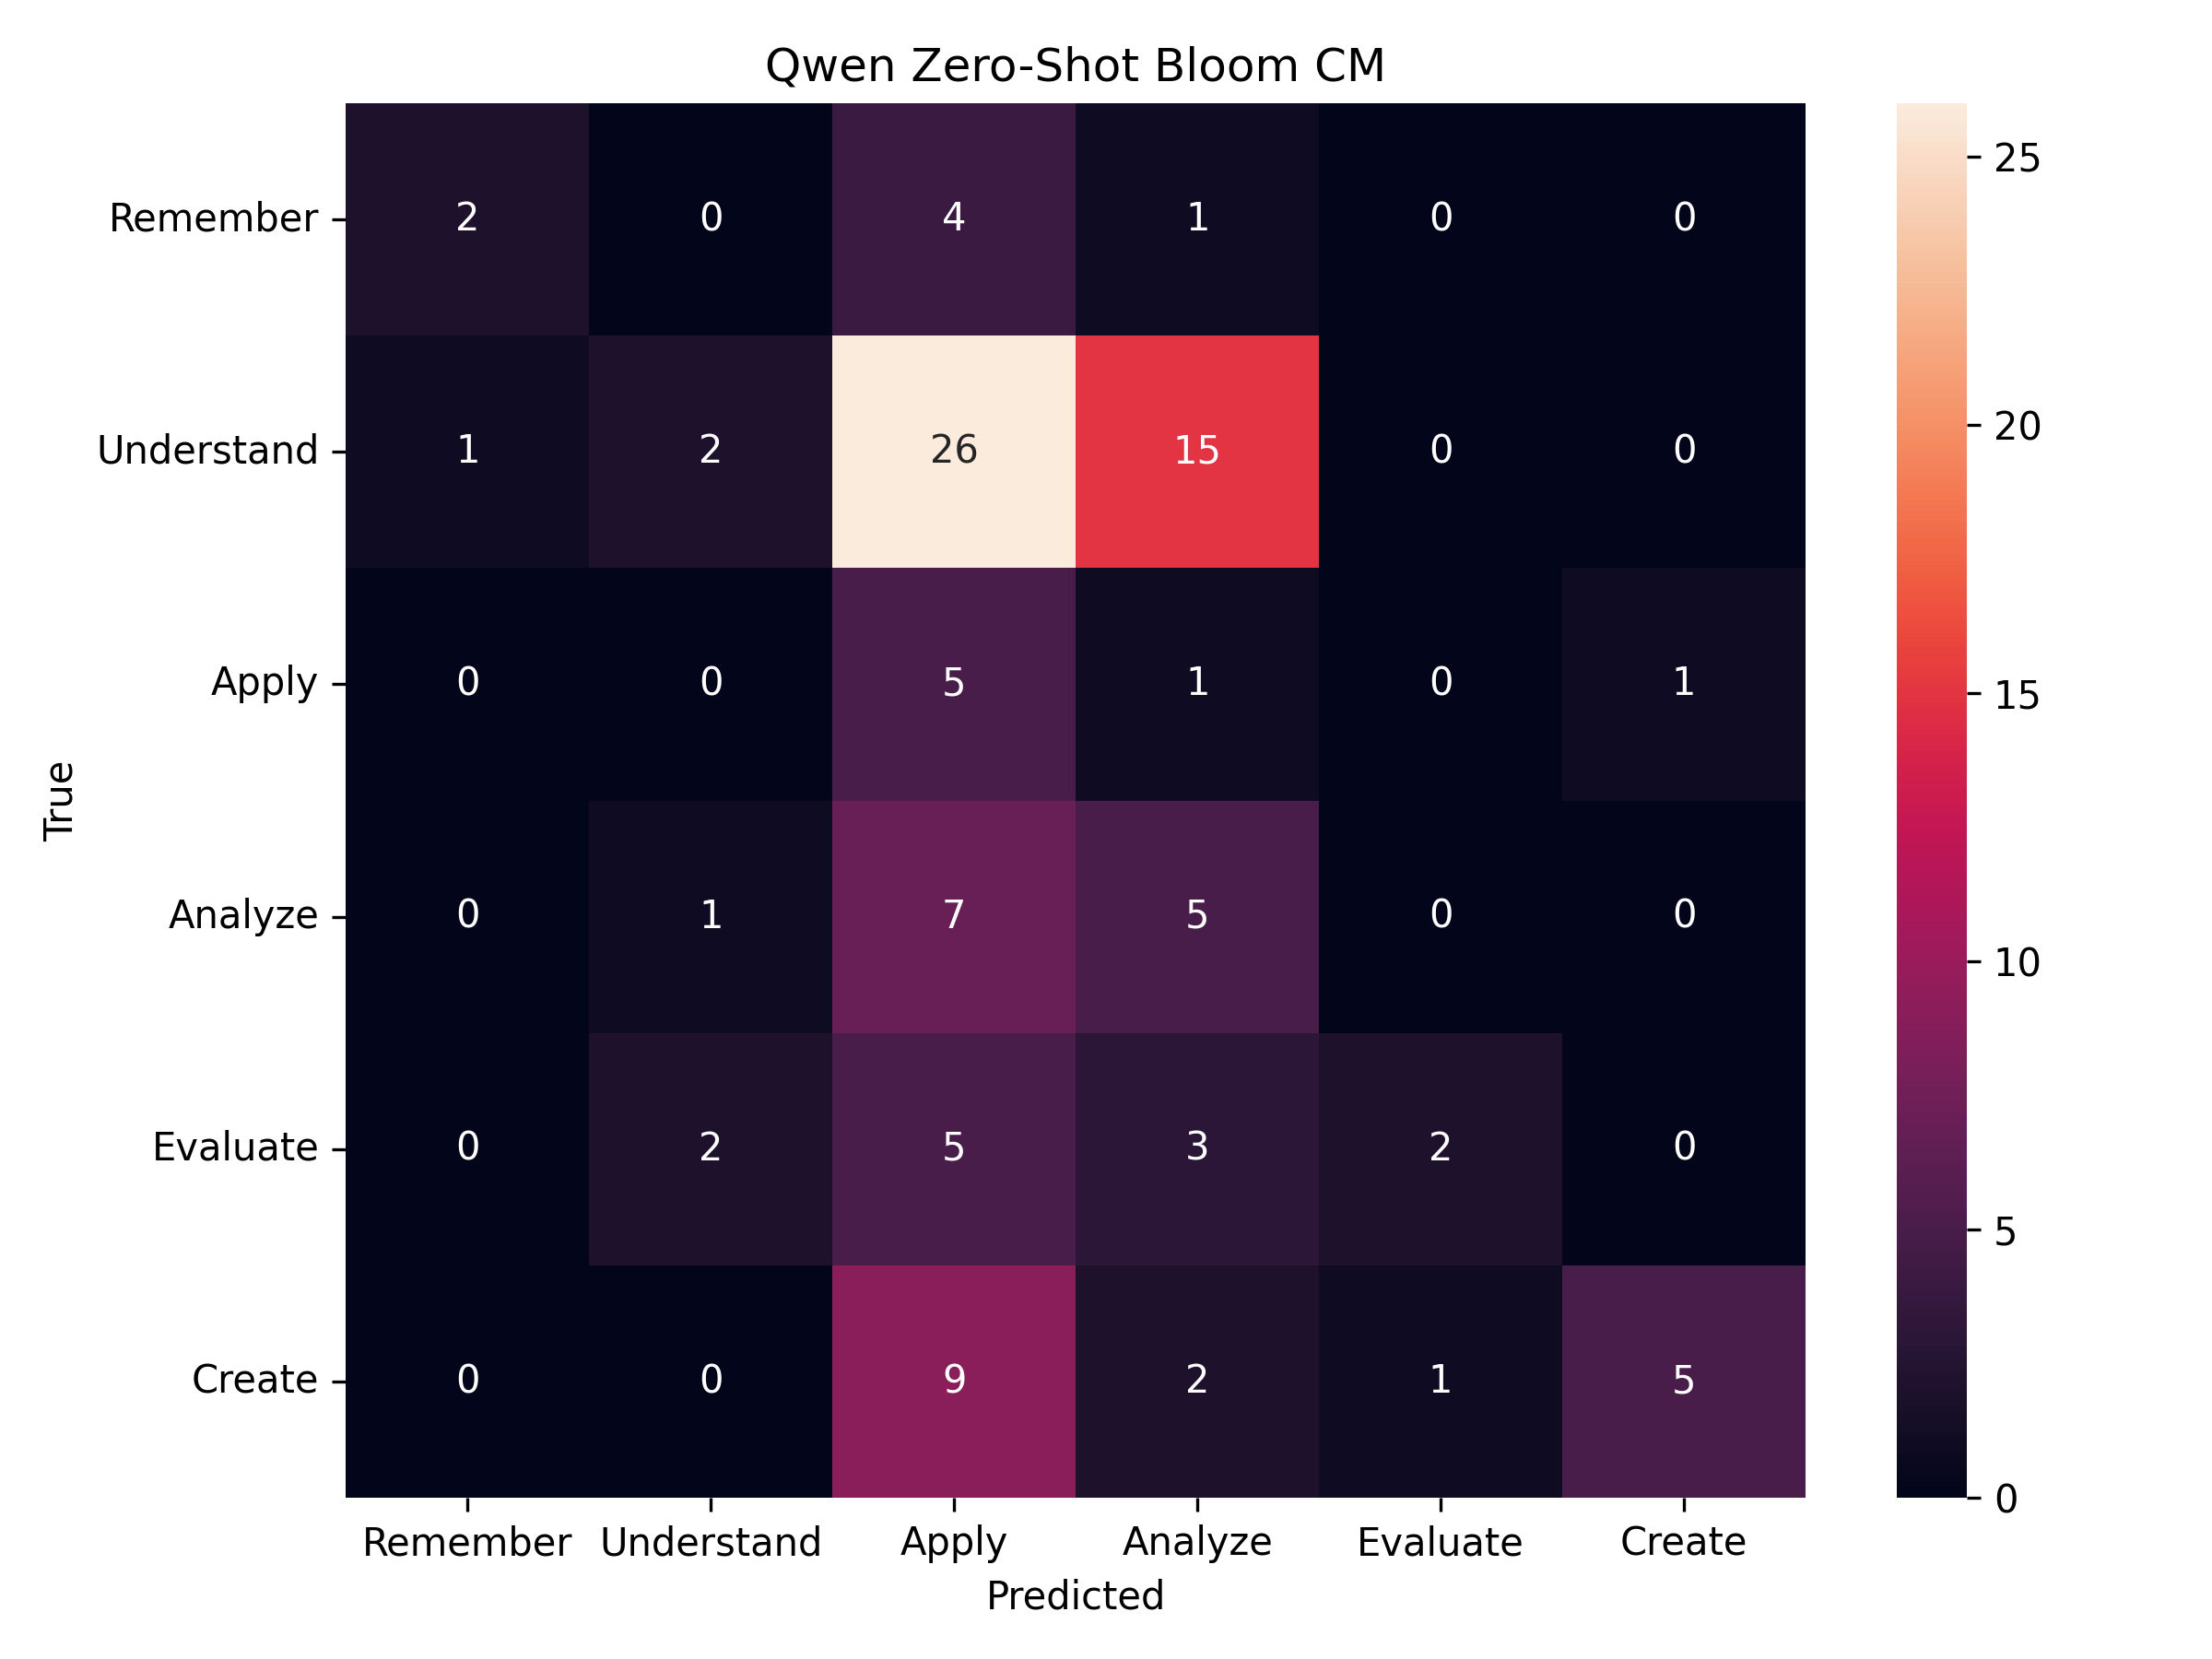
\includegraphics[width=\linewidth]{images/bloom_zero_shot_cm.png}
    \caption{Zero-shot GGUF (hold-out)}
\end{subfigure}
\caption{Hold-out baseline confusion matrices.}
\label{fig:bloom_baselines_cm}
\end{figure}

\begin{figure}[H]
    \centering
    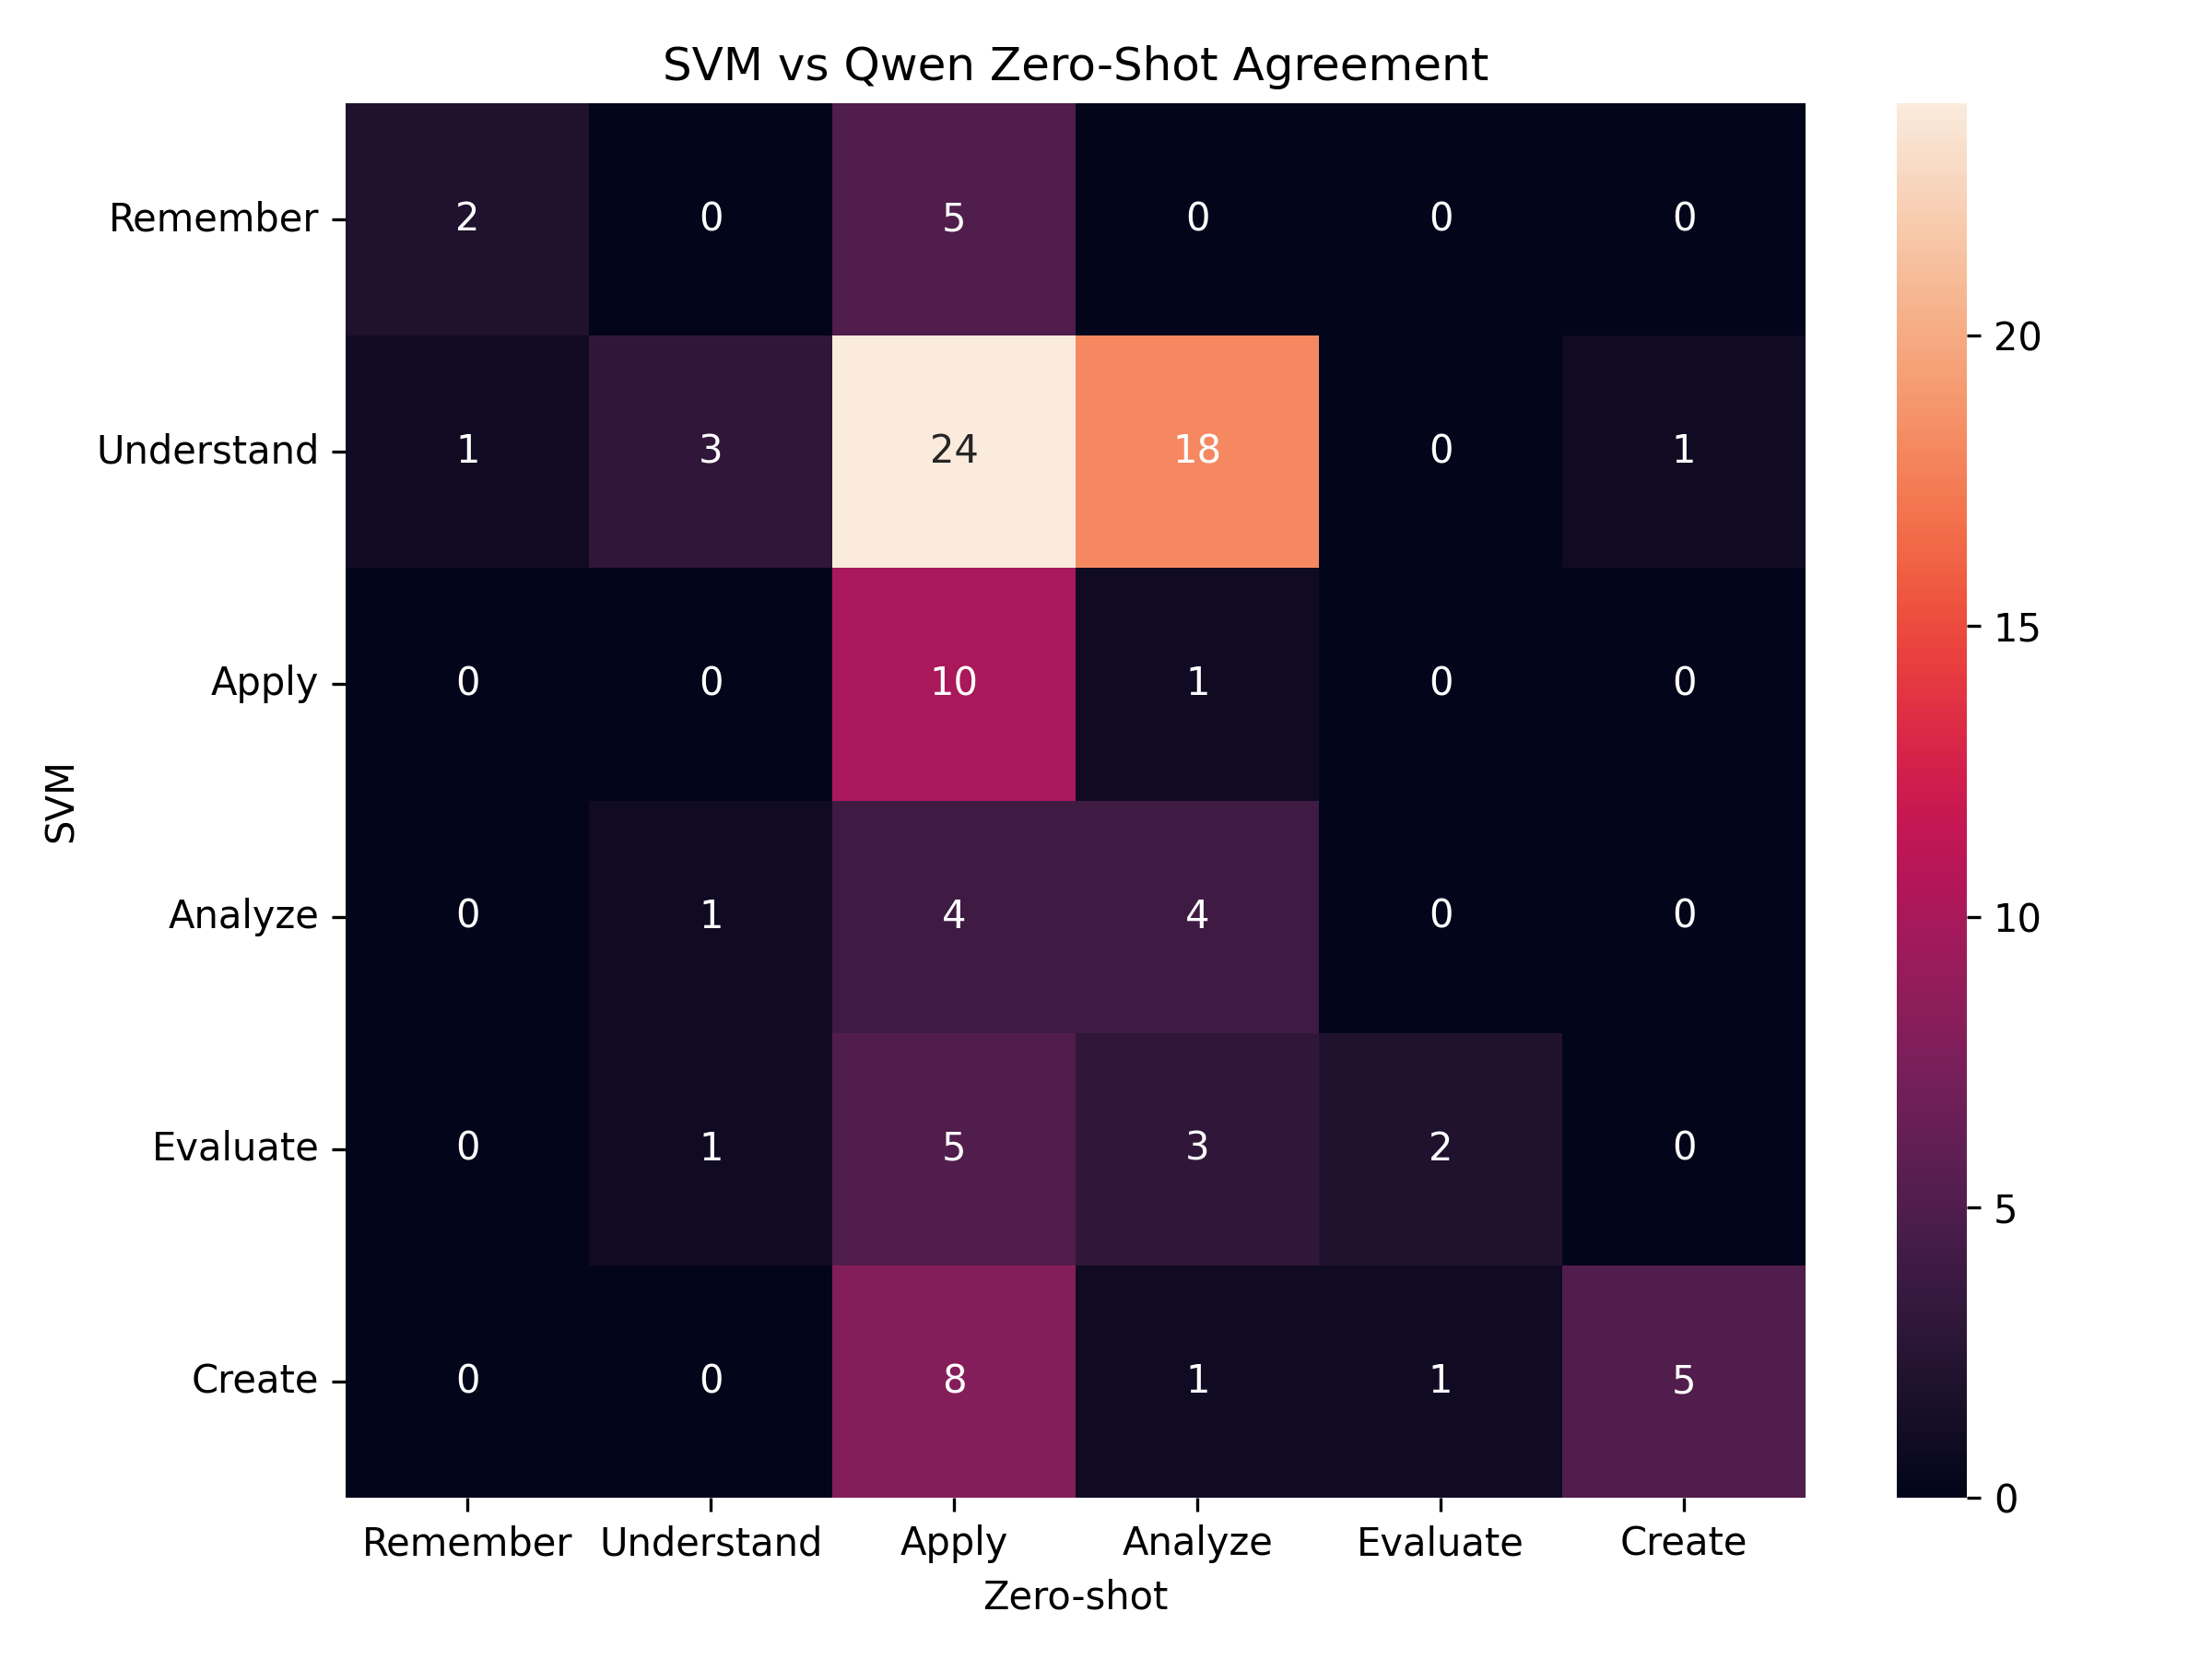
\includegraphics[width=0.75\textwidth]{images/bloom_svm_zero_shot_agreement.png}
    \caption{SVM vs.\ zero-shot label agreement (hold-out split).}
    \label{fig:bloom_agreement}
\end{figure}

\subsection{Role-Aware Privacy Guard}

The privacy evaluation uses 125 total rows: 104 student attack prompts, 15 benign student prompts, and 6 teacher moderation prompts. All evaluated student reconstruction attacks are blocked. Benign student prompts are allowed at 0.867, and teacher moderation prompts are allowed at 1.000.

\begin{table}[H]
\centering
\small
\caption{Role-aware privacy evaluation}
\label{tab:privacy_report}
\begin{tabular}{@{}lcc@{}}
\toprule
\textbf{Prompt group} & \textbf{Count} & \textbf{Rate}\\
\midrule
Student reconstruction attacks blocked & 104 & 1.000\\
Benign student prompts allowed & 15 & 0.867\\
Teacher moderation prompts allowed & 6 & 1.000\\
\bottomrule
\end{tabular}
\end{table}

\begin{figure}[H]
    \centering
    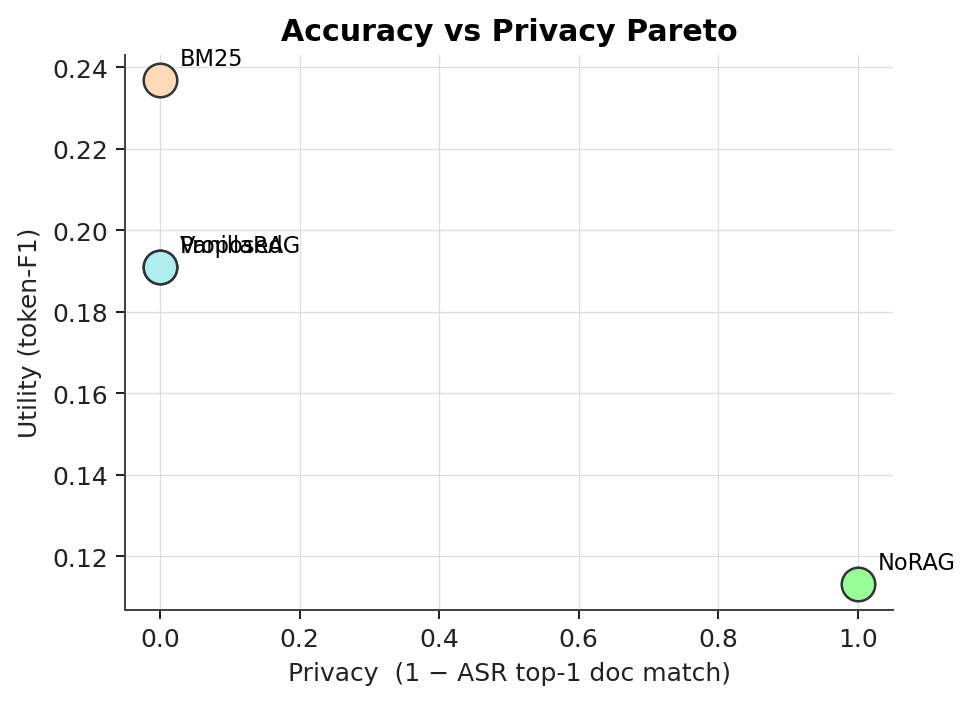
\includegraphics[width=0.75\textwidth]{images/accuracy_privacy_pareto.png}
    \caption{Accuracy/privacy trade-off (evaluation artifacts).}
    \label{fig:privacy_pareto_report}
\end{figure}

\subsection{Qwen GGUF: Student QA and RAG}

The student-facing stack uses \qwenmodel{}.gguf via llama.cpp (CPU-only, 986\,MB weights). Table~\ref{tab:qwen_rag_report} reports the ten-item academic QA benchmark (\texttt{results/qwen\_rag\_eval.json}).

\begin{table}[H]
\centering
\small
\caption{Qwen GGUF academic QA / RAG results ($n{=}10$)}
\label{tab:qwen_rag_report}
\begin{tabular}{@{}lrrr@{}}
\toprule
\textbf{Metric} & \textbf{Mean} & \textbf{Min} & \textbf{Max} \\
\midrule
Token-F1 & 0.914 & 0.471 & 1.000 \\
Exact match & 0.800 & 0.000 & 1.000 \\
Retrieval hit@1 & 0.900 & 0.000 & 1.000 \\
Retrieval hit@3 & 1.000 & 1.000 & 1.000 \\
Unsupported-answer proxy & 0.000 & 0.000 & 0.000 \\
\bottomrule
\end{tabular}
\end{table}

Extractive RAG ablations on the same benchmark: Proposed retriever token-F1 0.973 and exact match 0.900; VanillaRAG and BM25 match on F1/EM; NoRAG token-F1 0.025 (no retrieved context).

\begin{table}[H]
\centering
\footnotesize
\caption{RAG ablation comparison (same benchmark)}
\label{tab:qa_ablation_report}
\adjustbox{width=\textwidth,center}{%
\begin{tabular}{@{}lrrrrr@{}}
\toprule
\textbf{System} & \textbf{F1} & \textbf{EM} & \textbf{H@1} & \textbf{H@3} & \textbf{Unsup.}\\
\midrule
Qwen GGUF & 0.914 & 0.800 & 0.900 & 1.000 & 0.000\\
Proposed & 0.973 & 0.900 & 0.900 & 1.000 & 0.000\\
VanillaRAG & 0.973 & 0.900 & 0.800 & 1.000 & 0.000\\
BM25 & 0.973 & 0.900 & 0.900 & 1.000 & 0.000\\
NoRAG & 0.025 & 0.000 & 0.000 & 0.000 & 1.000\\
\bottomrule
\end{tabular}%
}
\end{table}

\subsection{Multimodal and OCR Evaluation}

Qwen multimodal RAG smoke tests pass PDF and image cases (answer accuracy 1.000 on two OK cases). OCR uses pytesseract: mean token-F1 0.963, WER 0.048, modality and access-level preservation 1.000 on synthetic typed images.

\begin{table}[H]
\centering
\small
\caption{OCR and multimodal ingestion}
\label{tab:ocr_report}
\begin{tabular}{@{}lc@{}}
\toprule
\textbf{Metric} & \textbf{Value}\\
\midrule
PDF RAG smoke test & Passed\\
Image RAG smoke test & Passed\\
Answer accuracy (OK cases) & 1.000\\
OCR backend & pytesseract\\
Mean OCR token-F1 & 0.963\\
Mean word error rate & 0.048\\
\bottomrule
\end{tabular}
\end{table}

\section{Comparison with Baseline / Existing Approaches}

Fine-tuned Qwen LoRA (0.748 accuracy) substantially outperforms zero-shot GGUF (0.441 on the hold-out split). TF-IDF + LinearSVC reaches 0.839 on that split, reflecting strong lexical cues; LoRA is preferred for deployment because it generalizes beyond surface patterns. For QA/RAG, NoRAG fails without retrieval; Qwen GGUF with FAISS retrieval achieves 0.914 token-F1.

\section{Discussion on Findings}

Role-separated corpora plus PrivacyGuard provide a practical university deployment pattern. Qwen LoRA delivers usable Bloom moderation; zero-shot Qwen classification alone is not adequate. Ordinal metrics show most LoRA errors are within one Bloom level.

\section{Limitations}

Synthetic privacy prompts, ten-item QA benchmark, typed-image OCR only, and simulated federated training. Formal differential privacy is not implemented.

\section{Summary}

Current metrics support deployable Qwen LoRA Bloom labeling, documented baselines, high attack block rate, and grounded Qwen GGUF RAG. See \texttt{results/unified\_results\_table.csv} and \texttt{results/bloom\_baseline\_comparison.json}.
